%%%%%%%%%%%%%%%%%%%%%%%%%%%%%%%%%%%%%%%%%
% Programming/Coding Assignment
% LaTeX Template
%
% This template has been downloaded from:
% http://www.latextemplates.com
%
% Original author:
% Ted Pavlic (http://www.tedpavlic.com)
%
% Note:
% The \lipsum[#] commands throughout this template generate dummy text
% to fill the template out. These commands should all be removed when 
% writing assignment content.
%
% This template uses a Perl script as an example snippet of code, most other
% languages are also usable. Configure them in the "CODE INCLUSION 
% CONFIGURATION" section.
%
%%%%%%%%%%%%%%%%%%%%%%%%%%%%%%%%%%%%%%%%%

%----------------------------------------------------------------------------------------
%	PACKAGES AND OTHER DOCUMENT CONFIGURATIONS
%----------------------------------------------------------------------------------------

\documentclass{article}

\usepackage{fancyhdr} % Required for custom headers
\usepackage{lastpage} % Required to determine the last page for the footer
\usepackage{extramarks} % Required for headers and footers
\usepackage[usenames,dvipsnames]{color} % Required for custom colors
\usepackage{graphicx} % Required to insert images
\usepackage{listings} % Required for insertion of code
\usepackage{courier} % Required for the courier font
\usepackage{verbatim} % For inserting actual code
\usepackage{hyperref} % For the hyperlinks

% Margins
\topmargin=-0.45in
\evensidemargin=0in
\oddsidemargin=0in
\textwidth=6.5in
\textheight=9.0in
\headsep=0.25in

\linespread{1.1} % Line spacing

% Set up the header and footer
\pagestyle{fancy}
\lhead{\hmwkAuthorName} % Top left header
\chead{\hmwkClass\ (\hmwkClassInstructor\ \hmwkClassTime): \hmwkTitle} % Top center head
\rhead{\firstxmark} % Top right header
\lfoot{\lastxmark} % Bottom left footer
\cfoot{} % Bottom center footer
\rfoot{Page\ \thepage\ of\ \protect\pageref{LastPage}} % Bottom right footer
\renewcommand\headrulewidth{0.4pt} % Size of the header rule
\renewcommand\footrulewidth{0.4pt} % Size of the footer rule

\setlength\parindent{0pt} % Removes all indentation from paragraphs

%----------------------------------------------------------------------------------------
%	CODE INCLUSION CONFIGURATION
%----------------------------------------------------------------------------------------

\definecolor{MyDarkGreen}{rgb}{0.0,0.4,0.0} % This is the color used for comments
\lstloadlanguages{Perl} % Load Perl syntax for listings, for a list of other languages supported see: ftp://ftp.tex.ac.uk/tex-archive/macros/latex/contrib/listings/listings.pdf
\lstset{language=Perl, % Use Perl in this example
        frame=single, % Single frame around code
        basicstyle=\small\ttfamily, % Use small true type font
        keywordstyle=[1]\color{Blue}\bf, % Perl functions bold and blue
        keywordstyle=[2]\color{Purple}, % Perl function arguments purple
        keywordstyle=[3]\color{Blue}\underbar, % Custom functions underlined and blue
        identifierstyle=, % Nothing special about identifiers                                         
        commentstyle=\usefont{T1}{pcr}{m}{sl}\color{MyDarkGreen}\small, % Comments small dark green courier font
        stringstyle=\color{Purple}, % Strings are purple
        showstringspaces=false, % Don't put marks in string spaces
        tabsize=5, % 5 spaces per tab
        %
        % Put standard Perl functions not included in the default language here
        morekeywords={rand},
        %
        % Put Perl function parameters here
        morekeywords=[2]{on, off, interp},
        %
        % Put user defined functions here
        morekeywords=[3]{test},
       	%
        morecomment=[l][\color{Blue}]{...}, % Line continuation (...) like blue comment
        numbers=left, % Line numbers on left
        firstnumber=1, % Line numbers start with line 1
        numberstyle=\tiny\color{Blue}, % Line numbers are blue and small
        stepnumber=5 % Line numbers go in steps of 5
}

% Creates a new command to include a perl script, the first parameter is the filename of the script (without .pl), the second parameter is the caption
\newcommand{\perlscript}[2]{
\begin{itemize}
\item[]\lstinputlisting[caption=#2,label=#1]{#1.pl}
\end{itemize}
}

%----------------------------------------------------------------------------------------
%	DOCUMENT STRUCTURE COMMANDS
%	Skip this unless you know what you're doing
%----------------------------------------------------------------------------------------

% Header and footer for when a page split occurs within a problem environment
\newcommand{\enterProblemHeader}[1]{
\nobreak\extramarks{#1}{#1 continued on next page\ldots}\nobreak
\nobreak\extramarks{#1 (continued)}{#1 continued on next page\ldots}\nobreak
}

% Header and footer for when a page split occurs between problem environments
\newcommand{\exitProblemHeader}[1]{
\nobreak\extramarks{#1 (continued)}{#1 continued on next page\ldots}\nobreak
\nobreak\extramarks{#1}{}\nobreak
}

\setcounter{secnumdepth}{0} % Removes default section numbers
\newcounter{homeworkProblemCounter} % Creates a counter to keep track of the number of problems

\newcommand{\homeworkProblemName}{}
\newenvironment{homeworkProblem}[1][Problem \arabic{homeworkProblemCounter}]{ % Makes a new environment called homeworkProblem which takes 1 argument (custom name) but the default is "Problem #"
\stepcounter{homeworkProblemCounter} % Increase counter for number of problems
\renewcommand{\homeworkProblemName}{#1} % Assign \homeworkProblemName the name of the problem
\section{\homeworkProblemName} % Make a section in the document with the custom problem count
\enterProblemHeader{\homeworkProblemName} % Header and footer within the environment
}{
\exitProblemHeader{\homeworkProblemName} % Header and footer after the environment
}

\newcommand{\problemAnswer}[1]{ % Defines the problem answer command with the content as the only argument
\noindent\framebox[\columnwidth][c]{\begin{minipage}{0.98\columnwidth}#1\end{minipage}} % Makes the box around the problem answer and puts the content inside
}

\newcommand{\homeworkSectionName}{}
\newenvironment{homeworkSection}[1]{ % New environment for sections within homework problems, takes 1 argument - the name of the section
\renewcommand{\homeworkSectionName}{#1} % Assign \homeworkSectionName to the name of the section from the environment argument
\subsection{\homeworkSectionName} % Make a subsection with the custom name of the subsection
\enterProblemHeader{\homeworkProblemName\ [\homeworkSectionName]} % Header and footer within the environment
}{
\enterProblemHeader{\homeworkProblemName} % Header and footer after the environment
}

%----------------------------------------------------------------------------------------
%	NAME AND CLASS SECTION
%----------------------------------------------------------------------------------------

\newcommand{\hmwkTitle}{Assignment\ \#4} % Assignment title
\newcommand{\hmwkDueDate}{Saturday,\ April\ 9,\ 2016} % Due date
\newcommand{\hmwkClass}{CSCI B\ 565} % Course/class
\newcommand{\hmwkClassTime}{} % Class/lecture time
\newcommand{\hmwkClassInstructor}{Prof. Predrag} % Teacher/lecturer
\newcommand{\hmwkAuthorName}{Vivek Patani (vpatani)} % Your name

%----------------------------------------------------------------------------------------
%	TITLE PAGE
%----------------------------------------------------------------------------------------

\title{
\vspace{2in}
\textmd{\textbf{\hmwkClass:\ \hmwkTitle}}\\
\normalsize\vspace{0.1in}\small{Due\ on\ \hmwkDueDate}\\
\vspace{0.1in}\large{\textit{\hmwkClassInstructor\ \hmwkClassTime}}
\vspace{3in}
}

\author{\textbf{\hmwkAuthorName}}
\date{} % Insert date here if you want it to appear below your name

%----------------------------------------------------------------------------------------

\begin{document}

\maketitle

%----------------------------------------------------------------------------------------
%	TABLE OF CONTENTS
%----------------------------------------------------------------------------------------

%\setcounter{tocdepth}{1} % Uncomment this line if you don't want subsections listed in the ToC

\newpage
\tableofcontents
\newpage

%----------------------------------------------------------------------------------------
%	PROBLEM 1
%----------------------------------------------------------------------------------------

% To have just one problem per page, simply put a \clearpage after each problem

\begin{homeworkProblem}
Listing \ref{homework_example} shows the pseudocode.

\perlscript{homework_example}{Pseudocode}

\begin{itemize}

\item ROC can be generated with the help of classifier which predicts class of a data point and the posterior probability.

\item The idea is to find the minimum and maximum number of points to find the area under the ROC curve.

\item Let us see what the pseudocode says - We first sort the data points on basis of their probability picking each of the distinct probability as the thresholds. This can also sometimes indicate that the maximum number of threshold as n itself as probability of each data point can be taken as threshold.

\item The next step we initalise TP \& FP(True Positives and False Positives) as zero. As we go on they will be incremented as and when whatever occurs. We then create a Stack R which consists of all the ROC points. The observation also sees that the complexity of our algorithm is $O(n\log n)$.

\item Next step is to on until all the points are over. We also need to keep a check on the instances with equal probability.

\item When we enter the loop say for example if all the probabilities are equally likely, what happens then? There will be two extremes as either we will only end up having a single point since the if condition will not be TRUE at all.

\item Similarly just think that if all the probabilities are unique and unequal then too we will have n values causing us to think of the higher bound.

\item To summarise my answer I would say if and only if we have the starting and end point then we need only 1 point to plot the ROC and calculate area. Since I'm assuming we are known to have (0,0) and (1,1) then we can rely on a single point since it completes the curve, but if we have no prior knowledge then we might as well need a minimum of two points both on the opposite axis (For FP and TP). The maximum number of points that we need would be the number of unique posterior probability which may or may not equal to 1.
\end{itemize}

\end{homeworkProblem}
\clearpage

%----------------------------------------------------------------------------------------
%	PROBLEM 2
%----------------------------------------------------------------------------------------

\begin{homeworkProblem}

\perlscript{q2}{Pseudocode}
\begin{itemize}
\item The idea is to merge m pairs of clusters minimising SSE of all clusters.
\item In order to do that we need to start off with the number of clusters, for every cluster go to every other cluster and get the distance, store it.
\item Once both the for loops end we will get the list of shortest distance and pick up the smallest one.
\item The formula for SSE: \\$SSE_{C_xC_y}$=$\frac{1}{2|C_x|}\sum_{x \epsilon C_x}{\sum_{y \epsilon C_x}}dist(x,y)^2$ + $\frac{1}{2|C_y|}\sum_{x \epsilon C_y}{\sum_{y \epsilon C_y}}dist(x,y)^2$ + $\frac{1}{2|C_x+ C_y|}\sum_{x \epsilon C_x}{\sum_{y \epsilon C_y}}dist(x,y)^2$
\item We assume that the SSE is the average of all points in the cluster from the centre for a certain cluster.
\end{itemize}
\end{homeworkProblem}
\clearpage

%----------------------------------------------------------------------------------------

%----------------------------------------------------------------------------------------
%	PROBLEM 3
%----------------------------------------------------------------------------------------

\begin{homeworkProblem}

\problemAnswer{
\begin{center}
What are \textbf{Association Rules}?\\
\begin{itemize}
\item The idea of Association Rules is that it can be defined as a pattern stating the occurrence of one event, by which another event occurs with a certain probability.\\
\item In other words, they are simple If/Else statements which help us discover patterns between unrelated data.\\
\item The interesting part of Association Rules is that they help us learn relationships of objects which are frequently collectively used.\\
\item The goal is to find all sets (only important ones) having \textit{support} \textgreater  \textit{minsup} (minimum support).
\item Followed by checking which rules cross a certain level of confidence. It means that not all rules generated are important, instead simply pick those rules which have \textit{confidence} \textgreater \textit{minconf}.
\item The two most basic and important things to look out while mining Association Rules are \textbf{Support} \& \textbf{Confidence}. Also \textbf{Lift} is another alternative, due to the shortcomings of the prior.\\
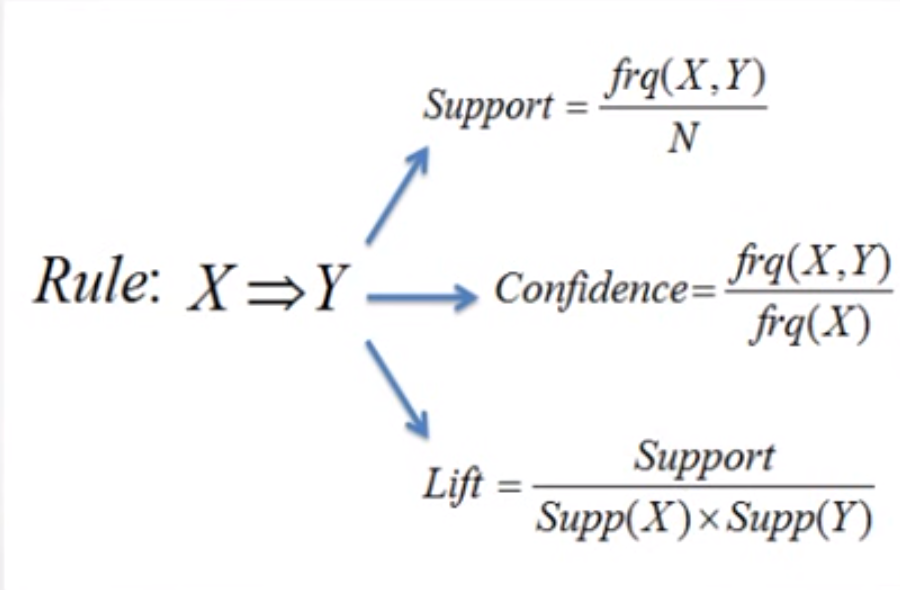
\includegraphics[width=0.75\columnwidth]{AssociationRules} % Example image
\item Some places where this is used is:
\begin{itemize}
\item Market Basket Analysis.
\item Medical Diagnosis
\item Protein Sequences
\item Census Data
\end{itemize}
\end{itemize}
\end{center}
}
\linebreak
The basic \textbf{Apriori Algorithm} is divided into two parts:\\
\begin{itemize}
\item Finding Frequent Itemsets.
\begin{itemize}
\item Generating Candidate Itemsets.
\item Filtering the useful candidates.
\end{itemize}
\item Mining/Discovering Unknown Patterns from frequent itemsets.
\end{itemize}
\begin{enumerate}
\item How to find the Frequent Itemsets?
\begin{itemize}
\item The very basic need is to specify a \textbf{Support level}.
\item Next step consists of actually scanning through the input transaction set and only collecting that cross the threshold of Support with 1 - item set in mind. In other words, eliminate those who do not matter and contribute towards forming interesting patterns.
\item Once we filter based on the support level, we start building candidate sets of k - items.
\item This is gradually done by combining 1 - item sets to form 2 item sets, moving onto three and so on until you do not find an empty set since none crossed the support threshold and k-1 set is returned.
\item So the set generated as C1 (Candidate 1) is filtered to become L1 or F1 (Frequent Sets), which in turn becomes C2 followed by filtering to become C3 and so on.
\item The preprocess.py contains the program to convert datasets to sparse matrix.
\item This is done with the help of two methods: \[F_k -1 * F_k -1\] \[F_k-1 * F_1\]
\item Implementation is done along with apriori in apriori.py (Answer to A part of question).
\item The First method generates lesser number of subsets compared to the latter one since the number of combinations are sorted lexicographically and then the combinations are made for those item sets who have k-2 elements in common at each level of iteration. So two generate a k=4, it's first two itemsets should have been the same to form a possible combination.
\item The Second method generates more item sets because of the fact even though they are sorted they are combined with Candidate 1 set. There is a better chance of duplication generation here rather than the prior method.
\item Once we find the possible combinations that make are possible, we then move to remove that do not make sense or rather that do not pass the \textbf{support threshold}.
\item Once we are through with this, then comes the rule generation. The frequent itemset is passed on to the next step.
\end{itemize}
\item How to find maximal and closed frequent itemsets?
\begin{itemize}
\item Implementation of C part is done in Misc-Max-Min.py
\item This is simple, starting from the top of the lattice just look for itemsets in the current level to be subsets of the item sets of next level, if they are subset then they are not maximal frequent item set. If they are not subsets they are meant to be maximal frequent itemset.
\item This is simple, starting from the top of the lattice just look for itemsets in the current level to have the same support as that of the item sets of lower level, if they have the same support count then they are not closed frequent item set. If they are not subset they are meant to be closed frequent itemset.
\item All the binarization (B part of the question) for each of the datasets is provided in the code file with the relevant dataset name followed by preprocessing \(eg: Nursery_preproccessing\). The Contraceptive dataset has three files, an additional to just convert numerical to categorical.
\item The result tells us that the size of Candidate $\geq$ Frequent $\geq$ Closed $\geq$ Maximal. The results below confirm to the principle.
\item This is the table for Nuresery dataset \url {https://archive.ics.uci.edu/ml/datasets/Nursery}
\[F_k -1 * F_k -1\]
\begin{center}
 \begin{tabular}{||c c c c c c||} 
 \hline
 Sr. No. & Support Value & Candidate & Frequent & Maximal & Closed\\ [0.5ex] 
 \hline\hline
 1 & 0.1 or 10\% & 822 & 166 & 113 & 164\\ 
 \hline
 2 & 0.01 or 1\% & 21813 & 6853 & 1683 & 2010\\
 \hline
 3 & 0.05 or 5\% & 2123 & 600 & 157 & 214\\ [1ex] 
 \hline
\end{tabular}
\end{center}
\item This is the table for Nuresery dataset \url {https://archive.ics.uci.edu/ml/datasets/Nursery}
\[F_k -1 * F_1\]
\begin{center}
 \begin{tabular}{||c c c c c c||} 
 \hline
 Sr. No. & Support Value & Candidate & Frequent & Maximal & Closed\\ [0.5ex] 
 \hline\hline
 1 & 0.1 or 10\% & 1106 & 166 & 113 & 164\\ 
 \hline
 2 & 0.01 or 1\% & 43422 & 6853 & 1683 & 2010\\
 \hline
 3 & 0.05 or 5\% & 4873 & 600 & 157 & 214\\ [1ex] 
 \hline
\end{tabular}
\end{center}
\item This is the table for Car dataset \url {https://archive.ics.uci.edu/ml/datasets/Car+Evaluation}
\[F_k-1 * F_1\]
\begin{center}
 \begin{tabular}{||c c c c c c||} 
 \hline
 Sr. No. & Support Value & Candidate & Frequent & Maximal & Closed\\ [0.5ex] 
 \hline\hline
 1 & 0.1 or 10\% & 315 & 86 & 43 & 50\\ 
 \hline
 2 & 0.01 or 1\% & 5383 & 2291 & 1000 & 1083\\
 \hline
 3 & 0.05 or 5\% & 1436 & 349 & 127 & 150\\ [1ex] 
 \hline
\end{tabular}
\end{center}
\item This is the table for Car dataset \url {https://archive.ics.uci.edu/ml/datasets/Car+Evaluation}
\[F_k-1 * F_k-1\]
\begin{center}
 \begin{tabular}{||c c c c c c||} 
 \hline
 Sr. No. & Support Value & Candidate & Frequent & Maximal & Closed\\ [0.5ex] 
 \hline\hline
 1 & 0.1 or 10\% & 475 & 86 & 43 & 50\\ 
 \hline
 2 & 0.01 or 1\% & 7104 & 2291 & 1000 & 1083\\
 \hline
 3 & 0.05 or 5\% & 1838 & 349 & 127 & 150\\ [1ex] 
 \hline
\end{tabular}
\end{center}
\item This is the table for Contraceptive dataset \url {https://archive.ics.uci.edu/ml/datasets/Contraceptive+Method+Choice}
\[F_k -1 * F_k-1\]
\begin{center}
 \begin{tabular}{||c c c c c c||} 
 \hline
 Sr. No. & Support Value & Candidate & Frequent & Maximal & Closed\\ [0.5ex] 
 \hline\hline
 1 & 0.1 or 10\% & 1937 & 767 & 166 & 406\\ 
 \hline
 2 & 0.01 or 1\% & 37634 & 21819 & 539& 834\\
 \hline
 3 & 0.05 or 5\% & 6243 & 2726 & 442 & 597\\ [1ex] 
 \hline
\end{tabular}
\end{center}
\item This is the table for Contraceptive dataset \url {https://archive.ics.uci.edu/ml/datasets/Contraceptive+Method+Choice}
\[F_k -1 * F_1\]
\begin{center}
 \begin{tabular}{||c c c c c c||} 
 \hline
 Sr. No. & Support Value & Candidate & Frequent & Maximal & Closed\\ [0.5ex] 
 \hline\hline
 1 & 0.1 or 10\% & 4962 & 767 & 166 & 407\\ 
 \hline
 2 & 0.01 or 1\% & 66771 & 21819 & 539 & 834\\
 \hline
 3 & 0.05 or 5\% & 13691 & 2726 & 442 & 597\\ [1ex] 
 \hline
\end{tabular}
\end{center}

\end{itemize}
\item Now we find the Association Rules, how do we do that?
\begin{itemize}
\item It is pretty straight forward. We now know the number of frequent itemsets and the sets. All we need to see is that the frequent itemsets generated, how worthy are they to us in terms of association.
\item We now generate rules. The first step is to enumerate and split each item in the frequent itemset. Once we know each individual element, we go on to merge them again. But why merge when you are splitting? We need to leverage each combination and see that whether if that combination does make sense at all or not?
\item How do we make sense? We can make sense by calculation of confidence of lift. Confidence and Lift are the two different ways to evaluate the rule, i.e. by lift or checking of minimum confidence threshold.
\item While coding we check if there are more than two sets, we look to merge them.
\item There are two parts of a rule \textit{Antecedent}, which is on the left and \textit{consequent}, which is on the right.
\item That being said we calculate for each support, various confidence values.
\item Confidence based pruning refers to removal of rule based on the idea that a tree branch should not be generated in case if that rule does not qualify for the minimum confidence threshold.
\item This means that superset of the current rule branch cannot have more confidence and hence does not qualify for as a good rule.
\item Part D, E and F are implemented over a number of files. But just running the main with the dataset should provide you with the results as per your customisation.
\item D Part:\\
\begin{itemize}

\item This is the table for Nuresery dataset \url {https://archive.ics.uci.edu/ml/datasets/Nursery}
\begin{center}
 \begin{tabular}{||c c c c c||} 
 \hline
 Sr. No. & Support Value & Confidence & Rules Generated & Pruning\\ [0.5ex] 
 \hline
 1 & 0.01 or 1\% & 0.25 & 41235 & 6853\\ 
 \hline
 2 & 0.01 or 1\% & 0.5 & 33861 & 693\\
 \hline
 3 & 0.01 or 1\% & 0.75 & 31012 & 4\\ [1ex] 
 \hline
 4 & 0.10 or 10\% & 0.25 & 341 & 289\\ 
 \hline
 5 & 0.10 or 10\% & 0.5 & 337 & 16\\
 \hline
 6 & 0.10 or 5\% & 0.75 & 279 & 3\\ [1ex] 
 \hline
 7 & 0.25 or 25\% & 0.25 & 18 & 3\\ 
 \hline
 8 & 0.25 or 25\% & 0.5 & 7 & 3\\
 \hline
 9 & 0.25 or 25\% & 0.75 & 7 & 3\\ [1ex]
 \hline
\end{tabular}
\end{center}
\item This is the table for Car dataset \url {https://archive.ics.uci.edu/ml/datasets/Car+Evaluation}
\begin{center}
 \begin{tabular}{||c c c c c||} 
 \hline
 Sr. No. & Support Value & Confidence & Rules Generated & Pruning\\ [0.5ex] 
 \hline
 1 & 0.01 or 1\% & 0.25 & 9036 & 1593\\ 
 \hline
 2 & 0.01 or 1\% & 0.5 & 9010 & 43\\
 \hline
 3 & 0.01 or 1\% & 0.75 & 9010 & 8\\ [1ex] 
 \hline
 4 & 0.10 or 10\% & 0.25 & 137 & 118\\ 
 \hline
 5 & 0.10 or 10\% & 0.5 & 137 & 22\\
 \hline
 6 & 0.10 or 5\% & 0.75 & 137 & 7\\ [1ex] 
 \hline
 7 & 0.25 or 25\% & 0.25 & 6 & 6\\ 
 \hline
 8 & 0.25 or 25\% & 0.5 & 6 & 3\\
 \hline
 9 & 0.25 or 25\% & 0.75 & 6 & 3\\ [1ex]
 \hline
\end{tabular}
\end{center}
\item This is the table for Contraceptive dataset \url {https://archive.ics.uci.edu/ml/datasets/Contraceptive+Method+Choice}
\begin{center}
 \begin{tabular}{||c c c c c||} 
 \hline
 Sr. No. & Support Value & Confidence & Rules Generated & Pruning\\ [0.5ex] 
 \hline
 1 & 0.01 or 1\% & 0.25 & 4551 & 3679\\ 
 \hline
 2 & 0.01 or 1\% & 0.5 & 3474 & 1270\\
 \hline
 3 & 0.01 or 1\% & 0.75 & 3190 & 311\\ [1ex] 
 \hline
 4 & 0.10 or 10\% & 0.25 &  & 289\\ 
 \hline
 5 & 0.10 or 10\% & 0.5 & 255 & 143\\
 \hline
 6 & 0.10 or 5\% & 0.75 & 243 & 39\\ [1ex] 
 \hline
 7 & 0.25 or 25\% & 0.25 & 279 & 279\\ 
 \hline
 8 & 0.25 or 25\% & 0.5 & 255 & 143\\
 \hline
 9 & 0.25 or 25\% & 0.75 & 243 & 63\\ [1ex]
 \hline
\end{tabular}
\end{center}
\end{itemize}

\item Here are the top 10s and the lift execution screenshots in sorted order.\\
\begin{itemize}
\item For Nursery Dataset\\
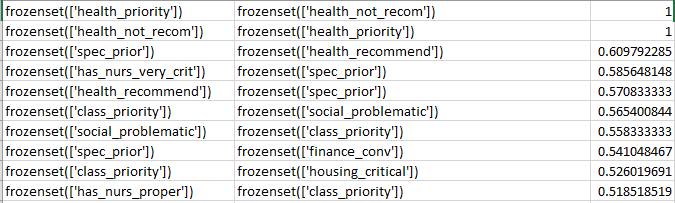
\includegraphics[width=0.75\columnwidth]{top10nursery.PNG}\\
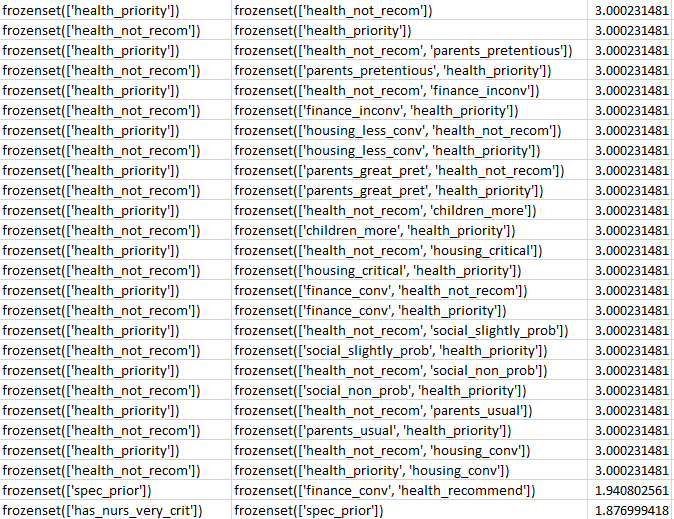
\includegraphics[width=0.75\columnwidth]{nurserylift.PNG}\\

\item For Car Dataset\\
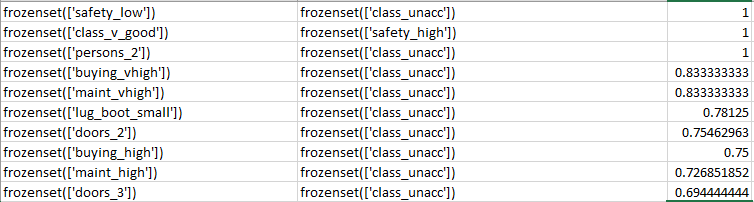
\includegraphics[width=0.75\columnwidth]{top10cars.png}\\
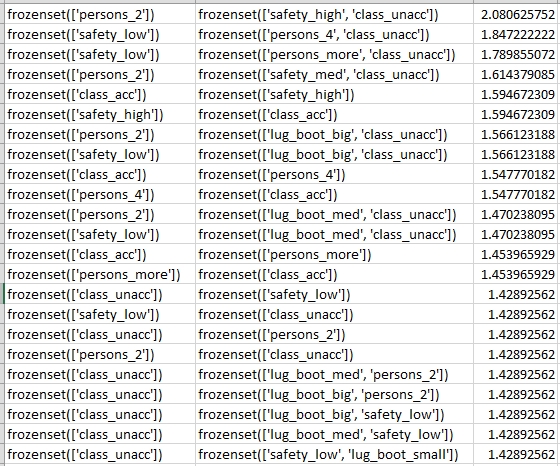
\includegraphics[width=0.75\columnwidth]{liftcar.PNG}\\

\item For Contraception Dataset\\
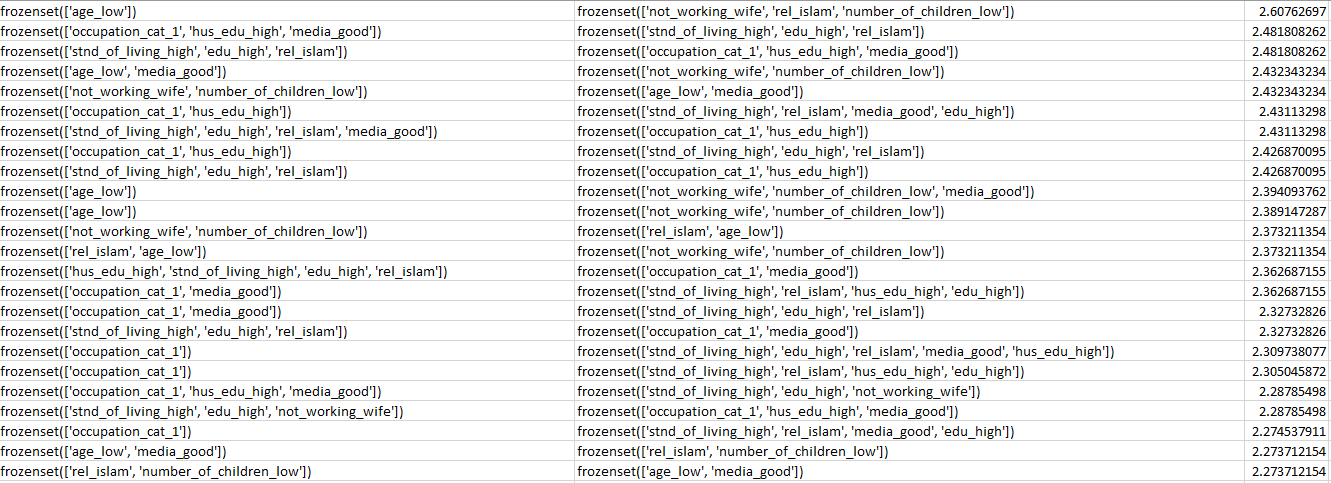
\includegraphics[width=0.75\columnwidth]{liftcmc.PNG}\\
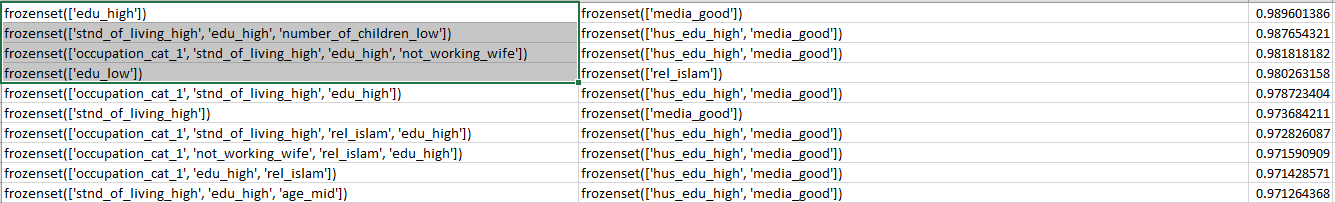
\includegraphics[width=0.75\columnwidth]{top10cmc.PNG}\\
\end{itemize}

\end{itemize}
\end{enumerate}

\end{homeworkProblem}
\newpage

%----------------------------------------------------------------------------------------
%	PROBLEM 4 A
%----------------------------------------------------------------------------------------

% To have just one problem per page, simply put a \clearpage after each problem

\begin{homeworkProblem}
\begin{center}
\textbf{Paper A}\\
\textbf{The idea of the paper}\\
The author mentions the study of clustering in this paper. He proposes the idea of a unified clustering of the objects and the difficulty in formulating a proposition which can be applied to all objects. He disproves the coexistence of three propositions because he then claims that there exist no such function which can satisfy those three properties of Scale Invariance, Richness and Consistency altogether. He displays the flaws in some algorithms which limit us to achieve the three aforementioned properties together.
\end{center}
\begin{itemize}
\item \textbf{Introduction}\\
The congregation of similar objects can be defined as Clusters. In other words, points having similar properties tend to be closer to each other than points they are less similar to forming clusters. Similar points in one cluster are less similar to points in other clusters. But that being said it should not be the only idea or aspect affecting the formation of a cluster, various accounts need to be considered while forming a cluster. The various axiomatic principles have been taken into account and their relation to the cluster properties that have been mentioned.

\item \textbf{The Impossibility Theorem}\\
The author talks about the restriction of distance metric which maybe distance and the triangular inequality property of a metric. Though he does not actually use it, it is of significant importance in understanding the other three properties. He mainly is talking about three properties:\\
\begin{enumerate}
\item Scale Invariance - The author checks the sensitivity of a function. He claims that the quantity of measure taken should not affect the result.\\
\begin{center}
$f(d) = f(\alpha d)$
\end{center}
\item Richness - The author here wants to say that the reconstruction of the output should be generated or can be generated by any partition and should be equally probable to be selected.
\item Consistency - This is one of the important and impactful property. The property talks about the consistency. It says that when intra cluster distance is appreciated and inter cluster distance is depreciated we should still obtain the same result. The author defines new variables $d$ \& $d'$, where $d$ is the original distance and then $d'$ is the  distance which is calculated after manipulation.
\end{enumerate}

\item \textbf{Claims}\\
The author now claims that if the  n greater than or equal 2 , then there exists no function that could satisfy the aforementioned properties. Before he proves this, the author shows the interrelation of these properties and shows that any two properties can be satisfied at one time but not three. The author takes into consideration the single linkage properties which says clusters can be represented as weighted graphs and sub graphs and defines three terminating conditions:

\begin{enumerate}
\item K - Cluster Property - When we achieve a graph of K connected components we terminate.
\item Distance R Property - Weights more than R should be avoided.
\item Scaling - alpha Property - P Indicates the max pairwise distance, weights of about scaled P is appended.
\end{enumerate}

\item Hence the conclusion based on the above mentioned terminating condition we confirm that only any two rules can be satisfied.

\item The various combinations that are possible:
\begin{itemize}
\item When K is greater than or equal to 1 and for any n greater than equal to K will only satisfy Properties 1 \& 3.
\item Any positive $\alpha$ along with scale $\alpha$ stopping condition satisfy 1 \& 2.
\item Finally for R greater than 0, and n greater than or equal to 2, 2 \& 3 are satisfied.
\end{itemize}

\item \textbf{Anitchains}\\
In order to prove it in a much consistent and solid manner we use a set of special refinement cluster. Let us understand by an example. Let us say that the resultant cluster is $A$ and $B$, then there exists a partition cluster $A'$ which will be a $A' \subseteq A$ and also $B' \subseteq A$. Once we prove this the author simply goes ahead and proves the proposition. He finds the flaws in the equation mentioned above. That is say if Scale and Consistency property are satisfied then the range function will form an \textbf{Antichain}. Similarly other two propositions are further strengthened.

\item \textbf{Centroid Based Clustering and Consistency}\\
The author in this part of the paper claims to have said that the \textbf{centroid} based algorithms do not or cannot satisfy the Consistency Property. He proposes to us the idea of a new method known as $(k,g)$-based centroid clustering method. This method does the selection of centroids from a set of already existing points which is then followed by assigning points to the closest centroid forming clusters.

\item \textbf{Relaxing Properties}\\
Here the author actually wants us to understand the idea of relaxation so that all the properties can be satisfied. He introduces the idea of Refinement Consistency saying that if $d'$ being a transformation of $f(d)$, then $f(d')$ should be a refined version of $f(d)$.

\item \textbf{My Understanding}\\
As far as my knowledge extends I have come to the conclusion that the Consistency property has a major role to play. If we could somehow introduce a function and relax the consistency property a little bit, we sure would be able to satisfy the other properties. The size of a cluster and the number of clusters also play a major role in the idea of satisfying all the properties (which is mentioned in the next paper), keeping in mind all this if only the author could expand his horizon and extend to something more than Clustering functions to find a solution to satisfy the properties.
\end{itemize}
~\\~\\~\\
\begin{center}
\textbf{Paper B}\\
\textbf{The idea of the paper}\\
This paper is in relation to the first paper mentioning the idea of \textbf{Impossibility Theorem}. The author discusses Cluster Qualities and opposes the claims made by in the first paper. She claims that the instead of defining the properties, let us work with the cluster quality without leading to any sort of inconsistencies. Clustering Quality can be best understood as a function which returns a non negative number representing how good the algorithm performs. Also she claims that impossibility is not an inherent feature but due to various assumed propositions it has become so.
\end{center}
\begin{itemize}

\item \textbf{Introduction}\\
In this paper the author introduces Clustering Quality Measure (CQM) which is independent of any specific algorithm and which she claims is much more general. This introduces the idea of comparing the result obtained by one algorithm with the result obtained by another, which gives us a common platform to compare them. Running time, as claimed by the author is Polynomial Time. The author then discusses the axioms and their weakness. The discussion takes into account as to on what grounds were the axioms proposed and how the consistency axiom is not good in terms of clustering functions. The author then on basis of the three basic properties prepares the first CQM after reformulating them.

\item \textbf{Relative Margin}\\
The author begins with defining the idea of Relative Point Margin. She says that relative margin is a mean of distances, where in when a point is selected we also select the closest center points followed by taking a ratio between them which is then appended to form a complete representative set. The realisation of a cluster to be good is to have a lower value of the ratio. The author then talks about the proposition by stating 3 lemmas in relation to properties.

\item \textbf{Soundness and Completeness}\\
The author in this part defines Completeness and Soundness which are meant to be compatible with the axioms. Soundness is something that says there should be consistency all the axioms, in other words it says that all the elements should be compatible with all the axioms. The term Completeness says that all the properties used by objects should be inherently followed by the axioms. She goes on to say that CQM tends to comply to the soundness and completeness properties, the clustering functions may fail.

\item \textbf{Isomorphism Invariance}\\
This axiom is interesting as it mentions the treating of each cluster with the same respect. Say two clusters are isomorphic if and only if there is preservation of distance between them. She says that there is indifference because a consistent set of CQM satisfies Isomorphism Invariance, Scale Invariance, Consistency and Richness.

\item \textbf{More about CQM}\\
\begin{itemize}
\item Weakest Link - The idea here is to see that points that do not belong to the same cluster are loosely packed while those in the same are tightly coupled with links among them. It is moreover the extremes or the longest links where in the emphasis is given to the longest links. Then the maximum value is selected and then is divided by the smallest distance between two clusters.

\item Additive Margin - Another example would be this, though it is a little different as it calculate the difference instead of the ratio as it considers the distance between two of its most closest cluster centres. It is the average of of Additive Point Margin averaging the intra cluster distance.
\end{itemize}

\item The author in the last part talks about the computational complexity. The author claims that the function is in terms of K and has polynomial complexity as $O(n^{k+1})$, but if centres are pre specified then they take lesser times, such that Relative Margin takes $O(nk)$ while Additive Margin takes $O(n^2)$ and Weakest Link takes $O(n^3)$. As mentioned earlier that number of clusters can play a major role while it is not discussed here. The authors the objective functions will fail to comply with the Scale Invariance and Richness but introduction of a new normalisation technique as said by the author can be used to overcome the issues. Another interesting thing the author mentions refinement preferring and coarsening preferring (they fail the richness property) which are quite similar to the previous papers annitchains. As they fail the richness property we again need to define the number of clusters while testing the quality of clusters using refinement.

\item \textbf{My Understanding}
The author convincingly disproves the impossibility theorem  and has with a very cogent study of how she went about doing that. The solution provided by the author in terms of CQM is a valid point but each method has their disadvantages. The idea of dependence on the number of clusters is the focal point and not always will CQM come through, I still would not be convinced that this method will work in all environments and on all objects and hence would still search for a method which would work ubiquitously. 

\end{itemize}
\end{homeworkProblem}
\clearpage

%----------------------------------------------------------------------------------------

%----------------------------------------------------------------------------------------
%	References
%----------------------------------------------------------------------------------------

\begin{center}
\title{References}
\begin{itemize}
\item \url{https://www.researchgate.net/publication/238525379_Association_rule_mining-_Applications_in_various_areas}
\item \url{https://www.youtube.com/watch?v=RHkvnRemaLE&index=3&list=PLVOXKA8fjRuvTVJt_n1rkRl6n3sGcyY6a}
\item \url{http://aimotion.blogspot.com/2013/01/machine-learning-and-data-mining.html}
\item \url{http://www2.ift.ulaval.ca/~chaib/IFT-4102-7025/public_html/Fichiers/Machine_Learning_in_Action.pdf}
\item \url{http://papers.nips.cc/paper/3491-measures-of-clustering-quality-a-working-set-of-axioms-for-clustering.pdf}
\item \url{http://www.cs.cornell.edu/home/kleinber/nips15.pdf}
\item \url{https://ccrma.stanford.edu/workshops/mir2009/references/ROCintro.pdf}
\end{itemize}
\end{center}
\clearpage

%----------------------------------------------------------------------------------------

\end{document}